\documentclass[11pt]{beamer}
\usetheme{Goettingen}
\usepackage[utf8]{inputenc}
\usepackage{amsmath}
\usepackage{amsfonts}
\usepackage{amssymb}
\usepackage{graphicx}
\usepackage{hyperref}
\usepackage[hang,flushmargin]{footmisc}

\author{Alex Heilman, Weiyi Gong, Qimin Yan}
\title{Machine Learning Applied to Materials Science}
\subtitle{Hypergraphs, Equivariant Networks, and Tensors}
%\setbeamercovered{transparent} 
%\setbeamertemplate{navigation symbols}{} 
%\logo{} 
\institute{Department of Physics, Northeastern University} 
%\date{} 
\addtobeamertemplate{navigation symbols}{}{%
    \usebeamerfont{footline}%
    \usebeamercolor[fg]{footline}%
    \hspace{1em}%
    \insertframenumber/\inserttotalframenumber
}


\usepackage[style=authortitle,backend=bibtex]{biblatex}
\addbibresource{chgcnn.bib}

\newenvironment{boxed2}
    {\begin{center}
    \begin{tabular}{|p{0.95\textwidth}|}
    \hline\\
    }
    { 
    \\\\\hline
    \end{tabular} 
    \end{center}
    }


\renewbibmacro*{\tiny cite:title}{\tiny%
  \printtext[bibhyperref]{%
    \printfield[citetitle]{labeltitle}%
    \setunit{\space}%
    \printtext[parens]{\printdate}%
  }%
}

\begin{document}

\begin{frame}
\titlepage
$\quad$ \includegraphics[scale=0.05]{nersc_logo.png} 
$\quad \quad\quad \ \ \ $\includegraphics[scale=0.2]{N.pdf}$\quad\quad\quad$
\includegraphics[scale=0.1]{doe_logo.png}
\end{frame}

%\begin{frame}
%\tableofcontents
%\end{frame}

\begin{frame}{Overview}
$\bullet$ Crystal graphs, MPNNs, and hypergraphs

\vspace{0.6cm}\pause

$\bullet$ Equivariant Networks and Tensors
\end{frame}


\section{Crystal Hypergraphs}
\begin{frame}{Crystal Graph Construction}

Usually represent crystalline systems as graphs (nodes and edges) \footcite{cgcnn}:

\begin{center}

\includegraphics[scale=0.7]{crystalgraph2.pdf}\pause
\end{center}

$\bullet$ Atoms are nodes

\medskip

$\bullet$ Edges denote 'neighbors'; based on distance

\medskip

$\bullet$ Feature vectors
\end{frame}

\begin{frame}{Message Passing on Graphs}

MPNN framework  \footcite{mpnn}:\pause
\begin{center}
\medskip
\begin{columns}
\begin{column}{0.52\textwidth}
$\bullet$ Message $m$ for each node $i$:

\vspace{1.53cm}

$\bullet$ Update function $U$ for layer $t$:
\end{column}
\begin{column}{0.45\textwidth}
$$
m_i^{t+1}=\sum_{n_j\in \mathcal{N}(i)} M_t(n_i^{t},e_{ij},n_j^t )
$$

$$
n_i^{t+1}=U_t(n_i^t,m_i^{t+1})
$$
\end{column}
\end{columns}

\vspace{1cm}\pause

We'll need to generalize this later...
\end{center}
\end{frame}

\begin{frame}{Graph Limitations}
Problem: \pause Graph encodes ONLY interatomic distances!\pause

\medskip 

\begin{center}

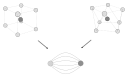
\includegraphics[scale=0.7]{crystalgraph_cntex.pdf}

\end{center}

These two crystalline structures have same representations!
\end{frame} 


\begin{frame}{Solution: Hypergraphs!}
Hypergraphs allow us to have larger hyperedges.\pause 

\vspace{.5cm}

\begin{center}
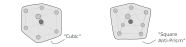
\includegraphics[scale=0.52]{crystalgraph_cntex_3.pdf}
\end{center}

\vspace{.5cm}

So we may define hyperedges for this local geometry.
\end{frame}


\begin{frame}{Local Environments as Hyperedges}
\small

Construct a hyperedge for each atom's entire local environment:

\medskip

\hspace{1cm}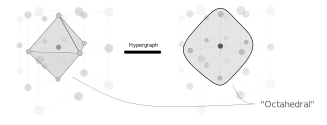
\includegraphics[scale=0.27]{motif_level_ex.pdf}

\medskip\pause

These contain the entire first shell of neighbors. \pause 

\medskip

$\bullet$ Geometry is encoded quantitatively with continuous symmetry measures or structure order parameters \footcite{orderparam1} as features 
\end{frame}

\begin{frame}{{\small Another Example:} Triplets as Hyperedges}


\begin{center}
Many modern models utilize bond angle information \footcite{alignn, m3gnet}. 

\medskip

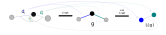
\includegraphics[scale=0.55]{line_graph_ex.pdf}


This is edge feature in a derived, auxiliary, 'line-graph'.

\medskip\pause


For hypergraphs, this is simpler:\pause

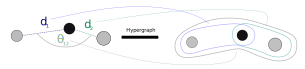
\includegraphics[scale=0.3]{triplet_ex.pdf}


\end{center}

\end{frame}


%\begin{frame}{Determining environments}
%To define a local environment, we need a way to systematically determine this environment for the relevant center sites.

%The determination of coordination environments often relies on the minimum distance between nearest neighbors for a site; and the largest solid angle spanned by a neighbors face in a Voronoi tesselation of the structure.
%\end{frame}


%\begin{frame}{Unit Cells as Hyperedges}
%Another order of hyperedge one may consider is that %describing the entire unit cell of some crystalline %structure. 

%A natural feature to encode in this cell-sized hyperedge is the point group of the system. 
%\end{frame}

%%%%%%%%%%%%%%%%%%%%%%%%%%%%%%%%%%%%%%%%%%%%%%%%%%%%%%%%%%5
%1
\begin{frame}{Crystal Hypergraphs}


\begin{center}
\includegraphics[scale=0.7]{hypergraph.pdf}
\end{center}
\vspace{.5cm}

\medskip

$\bullet$ In crystal hypergraph, all different order structures are on equal footing: bonds

\end{frame}

%2
\begin{frame}{Crystal Hypergraphs}


\begin{center}
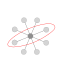
\includegraphics[scale=0.7]{hypergraph_2.pdf}
\end{center}
\vspace{.5cm}

\medskip

$\bullet$ In crystal hypergraph, all different order structures are on equal footing: bonds, triplets

\end{frame}
%3
\begin{frame}{Crystal Hypergraphs}


\begin{center}
\includegraphics[scale=0.7]{hypergraph_3.pdf}
\end{center}
\vspace{.5cm}

\medskip

$\bullet$ In crystal hypergraph, all different order structures are on equal footing: bonds, triplets, motifs

\end{frame}
%4
\begin{frame}{Crystal Hypergraphs}


\begin{center}
\includegraphics[scale=0.7]{hypergraph_4.pdf}
\end{center}
\vspace{.5cm}

\medskip

$\bullet$ In crystal hypergraph, all different order structures are on equal footing: bonds, triplets, motifs

\medskip

$\bullet$ Each has hyperedge type with invariant features: distance
\end{frame}

%5
\begin{frame}{Crystal Hypergraphs}

\begin{center}
\includegraphics[scale=0.7]{hypergraph_5.pdf}
\end{center}
\vspace{.5cm}

\medskip

$\bullet$ In crystal hypergraph, all different order structures are on equal footing: bonds, triplets, motifs

\medskip

$\bullet$ Each has hyperedge type with invariant features: distance, angle
\end{frame}

%6
\begin{frame}{Crystal Hypergraphs}


\begin{center}
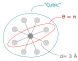
\includegraphics[scale=0.7]{hypergraph_6.pdf}
\end{center}
\vspace{.5cm}

\medskip

$\bullet$ In crystal hypergraph, all different order structures are on equal footing: bonds, triplets, motifs

\medskip

$\bullet$ Each has hyperedge type with invariant features: distance, angle, shape\pause

\begin{center}
But..... how do we update these representations?
\end{center}
\end{frame}

\begin{frame}{Extending Message Passing to Hypergraphs}

In the case of hypergraphs, neighborhood of nodes relevant to each message is now a set: \pause

\begin{gather*}
m_i^{t+1}=\sum_{h_j\ni n_i} M_t(n_i^{t},\underbrace{h_j^{t},\lbrace  n_w^t \vert n_w \in h_j }_{e_{ij},n_j}\rbrace)\\
\\
n_i^{t+1}=U_t(n_i^t,m_i^{t+1})\\
\end{gather*}

\begin{center}



\end{center}

\end{frame}



\begin{frame}{Comparative Performance Testing}
$\bullet$ We implement a basic convolutional structure amenable for (\textbf{3})
\vspace{1cm}\pause

$\bullet$ We focus on models with bond hyperedges and motif hyperedges.

\vspace{1cm}\pause

$\bullet$ Acts as testbed for what features/order correlations are most important for task.

\end{frame}

\begin{frame}{Hyperparameters and Model Architecture}
For each convolutional structure, testing was done for a model with 3 convolutional layers, an initial learning rate of 0.01, hidden node features of dimension 64, and a hidden output layer of dimension 128 (Similar to CGCNN's architecture). The loss function utilized is MSE.

\medskip

Datasets are split 80\% for training and 20\% for validation tests. 

\end{frame}

\begin{frame}{Materials Projet Datasets}\small
Below are results for various regression and classifications tasks for 152,605 materials.
\begin{center}


\medskip

\textbf{Formation Energy}

\begin{tabular}{c|ccc}
Model & Best MAE (eV/Atom) \\
\hline
Bond-only & 0.177 \\
Motif-only &  0.088 \\
Bond \& Motif &  \textbf{0.074} \\
\end{tabular}

\medskip

\medskip

\textbf{Band Gap}

\begin{tabular}{c|ccc}
Model & Best MAE (eV)  \\
\hline
Bond-only & 0.315 \\
Motif-only & 0.387  \\
Bond \& Motif & \textbf{0.301 }\\
\end{tabular}

\medskip

\medskip

\textbf{Metal/Non-metal}

\begin{tabular}{c|ccc}
Model & Best Accuracy  \\
\hline
Bond-only & .837\\
Motif-only & .853\\
Bond \& Motif & \textbf{.860}\\
\end{tabular}
\end{center}
\end{frame}

\begin{frame}{MatBench Datasets}\small
Below, we present results on validation sets for various MatBench target sets.


\begin{tabular}{c|ccc}
& Phonons (1,265) & Refractive Indices (4,764) \\
Model & Best MAE (cm$^{-1}$) & Best MAE \\
\hline
Bond-only & 78.9& \textbf{.4891}\\
Motif-only & 65.9& .5328\\
Bond \& Motif & \textbf{59.0}& .5222\\
\end{tabular}


\vspace{0.5cm}

\begin{tabular}{c|ccc}
& Perovskites (18,829)\\
Model & Best MAE (eV/Atom) \\
\hline
Bond-only & 0.329\\
Motif-only & \textbf{ 0.052}\\
Bond \& Motif & 0.058\\
\end{tabular}

\end{frame}
\begin{frame}{Overview of Experimental Results}\small

$\bullet$  Electronic tasks (band gap, dielectric targets) seem to benefit much less, or be negatively impacted, by this additional information. \pause It seems pair-wise correlators are, in general, a better descriptor for such tasks.

\vspace{.5cm}\pause

$\bullet$ Formation energy tasks benefit greatly from included motif (i.e. higher order geometrical) descriptors

\vspace{.5cm}\pause

$\bullet$ In the case of Perovskites (a harder set of formation energy targets), this geometrical information seems even more impactful\pause . Though, it also may just help more for the smaller dataset available for training.

\vspace{.5cm}\pause

$\bullet$ Phonons (also heavily dependent on geometrical information) seem to also benefit greatly from motif-level features

\vspace{.5cm}

\end{frame}




\begin{frame}{Conclusion}
$\bullet$ Graphs are limited in their expression of higher-order (above pair-wise) features of crystal structures

\vspace{.5cm}\pause

$\bullet$ Crystal hypergraphs give us a natural way to encode different types of features in one representation
\end{frame}

\section{Equivariance \& Tensors}
%\begin{frame}{Group Theory Background}
%A representation of a group is 
%\end{frame}

\begin{frame}{Equivariant Functions}
	An equivariant function $f:X\rightarrow Y$ is one that satisfies the following equality:
	$$
	f \big(D_X(g)\cdot x\big) = D_Y(g)\cdot f(x)
	$$
	
\end{frame}

\begin{frame}{Equivariant Convolution}
	Enforcing equivariance often restricts our choice of function; while also guaranteeing a natural condition for certain tasks.
	
	\medskip
	
	Hence, equivariance conditions may often restrict our trainable parameter space (requiring less data in training) while 
	providing similar expressibility of the model (giving similar, or sometimes better performance).
	
	\medskip
	
	
\end{frame}

\begin{frame}{Equivariant Convolution cont.}
	\begin{boxed2}
		\textbf{Example: Convolutional Networks and Translation}
		
		Traditional convolutional neural networks (CNNs) are actually equivariant under the group action of translation (in 2D for 
		the usual input of images).
	\end{boxed2}
\end{frame}

%\begin{frame}{Constructing Equivariant Filters}

%\end{frame}

\subsection{NEquiP}
\begin{frame}{Special Orthogonal Group in 3D}
	The special orthogonal group of 3 dimensions, $SO(3)$, is
	the group describing 3 dimensional rotations.
	
	It has irreducible representations indexed by a rotational order $\ell$ and a harmonic order $m$, termed the spherical harmonics $Y^{\ell}_m$.
	
	Note that products of spherical harmonics can be decomposed in terms of another linear superposition of spherical harmonics via Clebsch-Gordon Coefficients $C^{\ell_f  m_f}_{\ell_1  m_1\ell_2 m_2}$
	$$
	Y_{\ell_1}^{m_1}(\Omega)Y_{\ell_2}^{m_2}(\Omega)=\sum_{\ell_3, m_3}\sqrt{\frac{(2\ell_1+1)(2\ell_2+1)}{4\pi(2\ell_3+1)}}C^{\ell_3m_3}_{\ell_1m_1\ell_2m_2}C^{\ell_30}_{\ell_1 0\ell_2 0}Y_{\ell_3m_3}(\Omega)
	$$
\end{frame}

\begin{frame}{Tensor Field Networks/SO(3)}
	NEquiP utilizes a convolutional structure that is equivariant under the $SO(3)$ group, following that introduced in the Tensor Field Networks paper
	
	\vspace{1cm}
	
 	Layer-to-layer convolution defined as:
	$$
	\mathcal{L}_{acm_o}^{(l_o)} = \sum_{m_f,m_i} C_{l_fm_f,l_im_i}^{l_om_o}\sum_{b\in S}F_{cm_f}^{l_fl_i}(\vec{r}_{ab})V_{bcm_i}^{l_i}
	$$
\end{frame}





\begin{frame}{Hyperedge Index}
Computationally, we define a \textit{hyperedge index} of dimension 2 (as in previous hypergraph works):
\begin{align*}
[&[\text{node-index},...],\\
&[\text{hyperedge-index},...]]
\end{align*}
\end{frame}


\begin{frame}{Cell Hyperedges}
\small
Another order of hyperedge we may consider is that describing the entire unit cell of some crystalline structure.
\begin{center}
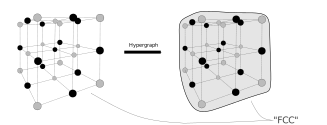
\includegraphics[scale=0.27]{cell_level_ex.pdf}
\end{center}
These 'unit' cell hyperedges allow for the explicit inclusion of global crystalline structure properties, i.e. point group information.

\medskip

This unit cell feature also may be learned through convolution and potentially used as a dynamic state vector.
\end{frame}




\begin{frame}{(Materials-Project) Formation Energy}\small
Below, validation MAE is shown through training for formation energy. The total dataset includes 152,605 materials.
\begin{center}

\includegraphics[scale=0.4]{formation_energy.png}

\medskip

\medskip


\begin{tabular}{c|ccc}
Model & Best MAE (eV/Atom) \\
\hline
Bond-only & 0.177 \\
Motif-only &  0.088 \\
Bond \& Motif &  \textbf{0.074} \\
\end{tabular}
\end{center}
\end{frame}
\begin{frame}{(Materials-Project) Band Gap}
Below are results for band gap training, based on a dataset including 152,605 materials.
\begin{center}\small
\includegraphics[scale=0.4]{band_gap.png}

\medskip

\begin{tabular}{c|ccc}
Model & Best MAE (eV)  \\
\hline
Bond-only & 0.315 \\
Motif-only & 0.387  \\
Bond \& Motif & \textbf{0.301 }\\
\end{tabular}
\end{center}
\end{frame}
\begin{frame}{(Materials-Project) Metal/Non-metal}
Below, we test metal/non-metal classification for 152,605 materials.
\begin{center}
\includegraphics[scale=0.4]{metal_nonmetal.png}

\medskip



\begin{tabular}{c|ccc}
Model & Best Accuracy  \\
\hline
Bond-only & .837\\
Motif-only & .853\\
Bond \& Motif & \textbf{.860}\\
\end{tabular}
\end{center}
\end{frame}

\begin{frame}{(MatBench) Perovskites}\small
Below, we test on 18,928 calculated formation energies for Perovskites.
\begin{center}
\includegraphics[scale=0.4]{perovskites.png}

\medskip


\begin{tabular}{c|ccc}
Model & Best MAE (eV/Atom) \\
\hline
Bond-only & 0.329\\
Motif-only & \textbf{ 0.052}\\
Bond \& Motif & 0.058\\
\end{tabular}
\end{center}
\end{frame}
\begin{frame}{(MatBench) Phonons}\small

Below, we test on a dataset of 1,265 materials with the target being the highest calculated frequency optical phonon mode peak.
\begin{center}

\includegraphics[scale=0.4]{phonons.png}

\medskip

\begin{tabular}{c|ccc}
Model & Best MAE (cm$^{-1}$) \\
\hline
Bond-only & 78.9\\
Motif-only & 65.9\\
Bond \& Motif & \textbf{59.0}\\
\end{tabular}
\end{center}
\end{frame}

\begin{frame}{(MatBench) Dielectrics}\small
Below, we test on the calculated refractive index of 4,764 materials
\begin{center}
\includegraphics[scale=0.43]{dielectric.png}

\medskip

\medskip
\begin{tabular}{c|ccc}
Model & Best MAE \\
\hline
Bond-only & \textbf{.4891}\\
Motif-only & .5328\\
Bond \& Motif & .5222\\
\end{tabular}
\end{center}
\end{frame}

\end{document}